\documentclass[a4paper,12pt]{article}

\usepackage{indentfirst}
\usepackage[utf8]{inputenc}
\usepackage{graphicx}
\usepackage{float}
\usepackage[portuguese]{algorithm2e}
\usepackage{amsmath}
\usepackage{xcolor}

\definecolor{pblue}{rgb}{0.13,0.13,1}
\definecolor{pgreen}{rgb}{0,0.5,0}
\definecolor{pred}{rgb}{0.9,0,0}
\definecolor{pgrey}{rgb}{0.46,0.45,0.48}

\usepackage{listings}
\lstset{language=Java,
	postbreak=\raisebox{0ex}[0ex][0ex]{\ensuremath{\color{red}\hookrightarrow\space}},
	numbers=left,
	xleftmargin=2em,
	frame=single,
	framexleftmargin=2em,
	showspaces=false,
	showtabs=false,
	breaklines=true,
	showstringspaces=false,
	breakatwhitespace=true,
	commentstyle=\color{pgreen},
	keywordstyle=\color{pblue},
	stringstyle=\color{pred},
	basicstyle=\scriptsize\ttfamily,
	moredelim=[is][\textcolor{pgrey}]{\%\%}{\%\%}
}
\title{Chat assíncrono criptografado utilizando  sockets TCP em Java}
\author{Sila Georges Agiru Judick Siebert\\UDESC
        \and Wagner Luis Sousa da Luz \\UDESC}
\date{\today}


\begin{document}

\maketitle

\begin{abstract}
Neste artigo, uma aplicação de bate-papo para enviar mensagens  criptografadas é proposta.
O algoritmo de criptografia é caracterizado por inverter valor dos bits da mensagem. A aplicação é desenvolvida usando a linguagem de programação Java e utilizando sockets TCP. A seguir são resumidas as etapas de engenharia de software seguidas durante a implementação deste projeto.
\end{abstract}


\section{Introdução}
Aplicativos de mensagens instantâneas tornaram-se populares sendo usados diariamente pelas pessoas. A maioria dos usuários convencionais na Internet não percebe que suas conversas estão sendo transmitidas em texto claro e são vulneráveis a espionagem durante a transmissão.
O projeto foi intitulado  chat assíncrono criptografado e seu objetivo principal é implementar uma sala de bate-papo com criptografia nas mensagens. Objetivos secundários foram a pesquisa sobre sockets e experiência prática dos autores no desenvolvimento de uma aplicação bate-papo baseada em Java utilizando conceitos de threads e sockets aprendidos em aula.
\subsection{Requisitos}
Nesta seção, descrevemos alguns dos requisitos gerais
do nosso aplicativo de sala de bate-papo distribuído.
\begin{itemize}
\item A criptografia deve inverter valor dos bits da mensagem.
\item Devem utilizar uma conexão TCP/IP.
\item Não utilizar a classe bufferedreader e bufferedwriter.
\end{itemize}



\section{A sua Implementação}
\subsection{Visão geral da aplicação}
\subsubsection{Estrutura}
A figura \ref{fig1} representa a estrutura da sala de bate-papo.
\begin{figure}[H]
	\centering
	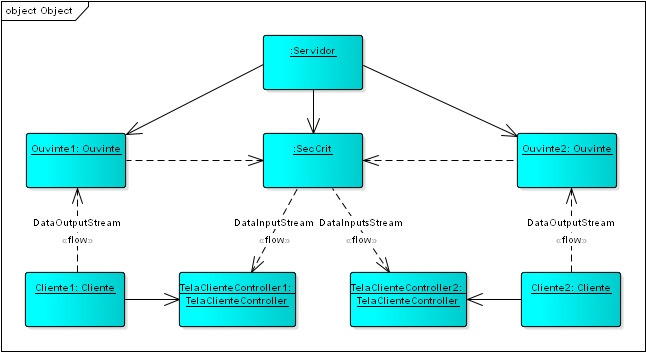
\includegraphics[scale=0.4]{img/objectdiagram.png}    
	\caption{Sala de bate-papo}
	\label{fig1}     
	\end{figure} 
\subsubsection{Diagramas de classe}
A figura \ref{fig2} representa o diagrama de classe da nossa implementação.
\begin{figure}[H]
	\centering
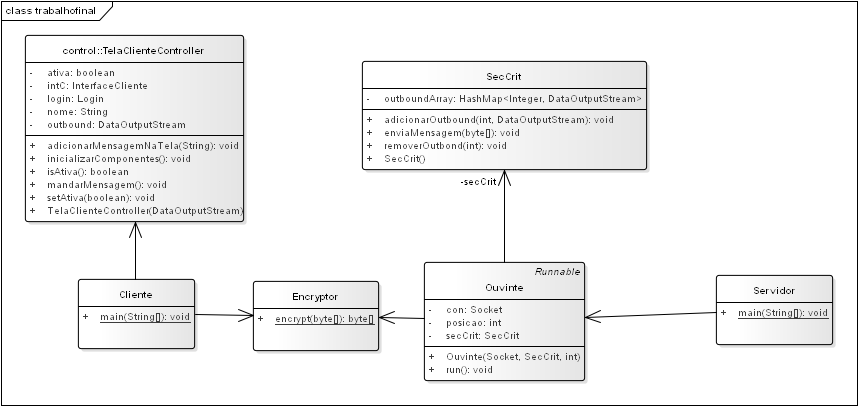
\includegraphics[scale=0.3]{img/class.png}    
\caption{Diagrama de classes da aplicação}

\label{fig2}
\end{figure} 
%\subsubsection{Diagramas de atividade}
%A figura \ref{fig3} representa o diagrama de atividade da classe servidor da nossa
%implementação.
%\begin{figure}[H]
%\centering
%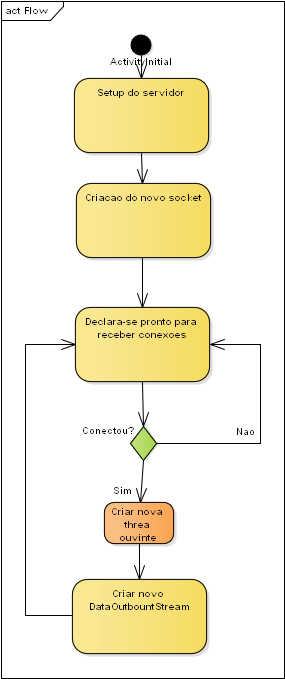
\includegraphics[scale=0.4]{img/serverflow.png}    
%\caption{Activity diagram do servidor}
%\end{figure}
%\subsection{Cliente}
\subsection{Cliente}
Cada cliente abre uma conexão TCP / IP para o servidor para envio e receber mensagens.
\begin{figure}[H]
	\lstinputlisting[firstline=14,lastline=16,frame=single]{../../TrabalhoFinal/src/trabalhofinal/Cliente.java}
	\caption{Conexão com o servidor - Classe Cliente}
\end{figure}
A tela do cliente deve ter um campo de texto no qual mensagens são exibidas à medida que chegam, e um campo para o usuário digitar mensagens de saída.
\begin{figure}[H]
	\centering
	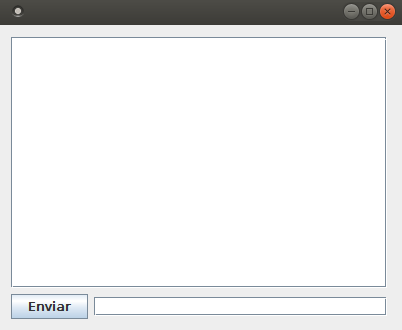
\includegraphics[scale=0.6]{img/telacliente.png}    
	\caption{Tela do cliente}
	\label{fig11}     
\end{figure} 
Cada mensagem deve ter a hora em que foi enviada,o nome do remetente, a mensagem decriptada e uma versão encriptada de mensagem. Qualquer número de pessoas deve ser capaz de participar.
\begin{figure}[H]
\lstinputlisting[firstline=21,lastline=37,frame=single]{../../TrabalhoFinal/src/trabalhofinal/Cliente.java}
\caption{Loop que recebe mensagens do servidor - Classe Cliente}
\end{figure}


\begin{figure}[H]
\lstinputlisting[firstline=78,lastline=81,frame=single]{../../TrabalhoFinal/src/trabalhofinal/control/TelaClienteController.java}
\caption{Método para mostrar a mensagem na tela - Classe TelaClienteController}
\end{figure}

\begin{figure}[H]
\lstinputlisting[firstline=59,lastline=76,frame=single]{../../TrabalhoFinal/src/trabalhofinal/control/TelaClienteController.java}
\caption{Metodo de envio de mensagens - Classe TelaClienteController}
\end{figure}

\subsection{Servidor}
O servidor aceita um cliente com a chamada ao accept,cria uma nova Thread Ouvinte para tratar cada cliente em sua própria Thread, logo adiciona um OutputStream dele e adiciona na lista de DataOutputStreams como podemos observar no código da Figura \ref{fig7}.Uma nova chamada ao accept aceita um novo cliente.
\begin{figure}[H]
\lstinputlisting[firstline=17,lastline=23,frame=single]{../../TrabalhoFinal/src/trabalhofinal/Servidor.java}
\caption{Método que recebe as conexões com os clientes - Classe Servidor}
\label{fig7}
\end{figure}
Agora que vários clientes podem mandar mensagens, gostaríamos que os clientes recebessem as mensagens enviadas pelos outros. Ao invés do servidor simplesmente escrever as mensagens no console, ele deve mandar cada mensagem para todos os clientes conectados.
\begin{figure}[H]
	\lstinputlisting[firstline=27,lastline=31,frame=single]{../../TrabalhoFinal/src/trabalhofinal/SecCrit.java}
	\caption{Método que distribui as mensagens para os clientes - Classe SecCrit}
	\label{fig8}
\end{figure}

Utilizando a lista de DataOutputStreams quando chegar uma mensagem, percorremos essa lista e mandamos uma mensagem a cada cliente individualmente.
\begin{figure}[H]
\lstinputlisting[firstline=30,lastline=50,frame=single]{../../TrabalhoFinal/src/trabalhofinal/Ouvinte.java}
\caption{Loop recebe mensagens do cliente - Classe Ouvinte}
\label{fig10}
\end{figure}


\subsection{Criptografia}
O algoritmo de criptografia é caracterizado por inverter valor dos bits da mensagem conforme ilustrado na Figura \ref{fig9}.
\begin{figure}[H]
\lstinputlisting[firstline=16,lastline=22,frame=single]{../../TrabalhoFinal/src/trabalhofinal/Encryptor.java}
\caption{Método que realiza a criptografia - Classe Encryptor}
\label{fig9}
\end{figure}


\section{Avaliação da implementação}
Ao lançar o servidor ele fica esperando conexões dos clientes. Quando um cliente se conecta ao servidor, este cria uma nova thread Ouvinte que fica “ouvindo” as mensagens desse cliente. 
Quando uma thread Ouvinte recebe uma mensagem de um cliente ela chama um método da classe SecCrit, a seção critica compartilhada por todas as threads ouvintes, passando a mensagem por parâmetro. Este método irá mandar a mensagem para todos os clientes percorrendo a lista de DataOutputstreams.
Quando um cliente manda uma mensagem contendo a palavra “adieu”(adeus em francês), o cliente é desconectado do servidor fechando a conexão, a thread ouvinte correspondente a este cliente chama o método para retirar o DataOutputStream da seção critica e fecha a thread.
Durante a implementação algumas dificuldades forma surgindo. A primeira deles sendo como manter todas as mensagens sincronizadas e na ordem em todas as janelas de bate-papo.
Outra dificuldade identificada foi reenviar as mensagens enviados de um cliente para o servidor, para todos os outros clientes.
A ultima dificuldade foi implementar a criptografia. Para isto algumas estrategias foram tentadas, nenhuma funcionando ate finalmente trabalhar somente com vetores de bytes.
\section{Conclusão}

A implementação do aplicativo forneceu uma excelente oportunidade para o uso prático de muitas das habilidades de projeto de software que os autores desenvolveram durante os últimos 3 anos na UDESC. O aplicativo atende às especificações funcionais conforme descrito nos requisitos deste relatório.
Atende ao principal objetivo de implementar uma sala de bate-papo com criptografia nas mensagens. Durante o desenvolvimento da aplicação os conceitos de sockets e threads foram aplicados na pratica e aprofundados, logo os objetivos secundários também foram atingidos.
%\bibliographystyle{plain}
%\bibliography{n2library.bib}

\end{document}
